% !TEX program = pdflatex
% Compile with: pdflatex aspirin_report.tex (run twice for refs)
% Or open in Overleaf and hit Recompile.

\documentclass[9pt]{extarticle}

\usepackage[margin=0.85in]{geometry}
\usepackage{amsmath}
\usepackage{graphicx}
\usepackage{float}
\usepackage{caption}
\usepackage{microtype}
\usepackage{enumitem}
\usepackage{parskip}
\usepackage{xcolor}
\usepackage[hidelinks]{hyperref}

\graphicspath{{images/}}

\captionsetup{font=footnotesize,labelfont=bf,skip=3pt}

\usepackage{titlesec}
\titlespacing*{\section}{0pt}{0.6\baselineskip}{0.2\baselineskip}
\titlespacing*{\subsection}{0pt}{0.4\baselineskip}{0.1\baselineskip}
\titleformat*{\subsection}{\bfseries\itshape}

\setlist{nosep,leftmargin=1.4em,topsep=2pt,parsep=2pt,partopsep=0pt}

\title{\vspace{-3em}Aspirin (Acetylsalicylic Acid): Structure, Synthesis, Reactivity, and Pharmacology}
\author{Abhinav Bachu \\ CHEM 332 / Organic Chemistry \\ Final Project --- Individual Submission}
\date{April 23, 2026}

\begin{document}
\maketitle
\vspace{-2.5em}

\section*{1: Compound Chosen}
Acetylsalicylic acid (\textbf{aspirin}), molecular formula
$\mathrm{C_9H_8O_4}$, molar mass $180.16~\mathrm{g\,mol^{-1}}$.
It is the acetyl ester of salicylic acid and is one of the most widely
used small-molecule drugs in the world, taken both for analgesia and as
a low-dose antiplatelet agent.

\begin{figure}[H]
\centering
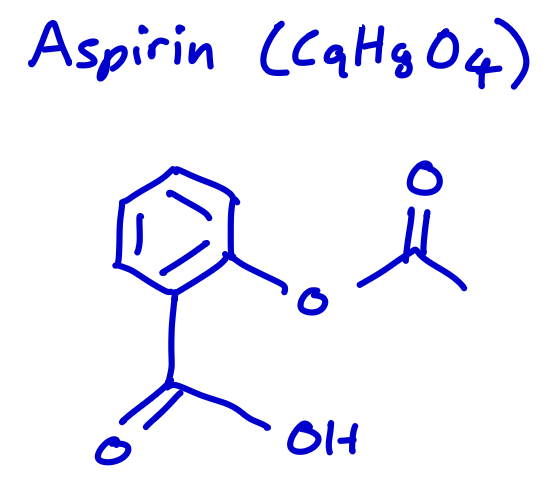
\includegraphics[width=0.24\linewidth]{img1.png}
\caption{CHEM~332\_Scheme~1. Skeletal structure of aspirin, $\mathrm{C_9H_8O_4}$.}
\label{fig:structure}
\end{figure}

\section*{2A: Structural Analysis}

\subsection*{Resonance Structures}
The chemically important set of contributors comes from the acetoxy
group's ester oxygen donating its lone pair into the aromatic ring
(Figure~\ref{fig:resonance}). The lone pair on \(\mathrm{O}\) can
either donate into the ester \(\mathrm{C{=}O}\)
(\(\mathrm{R{-}\ddot O{-}C{=}O}\leftrightarrow\mathrm{R{-}O^{+}{=}C{-}O^{-}}\))
or push \emph{through} the aryl C--O bond into the ring's $\pi$
system, placing negative charge at the ortho and para carbons (C3 and
C5). Two consequences: the acetoxy group acts as a weak $\pi$-donor /
o,p-director in EAS even though it is inductively electron-withdrawing
(Section~C), and the ester carbonyl is slightly less electrophilic
than a comparable ketone. The benzene Kekul\'e forms and the standard
\(\mathrm{C{=}O}\leftrightarrow\mathrm{C^{+}{-}O^{-}}\) carbonyl
resonance of the carboxylic acid contribute as well.

\begin{figure}[H]
\centering
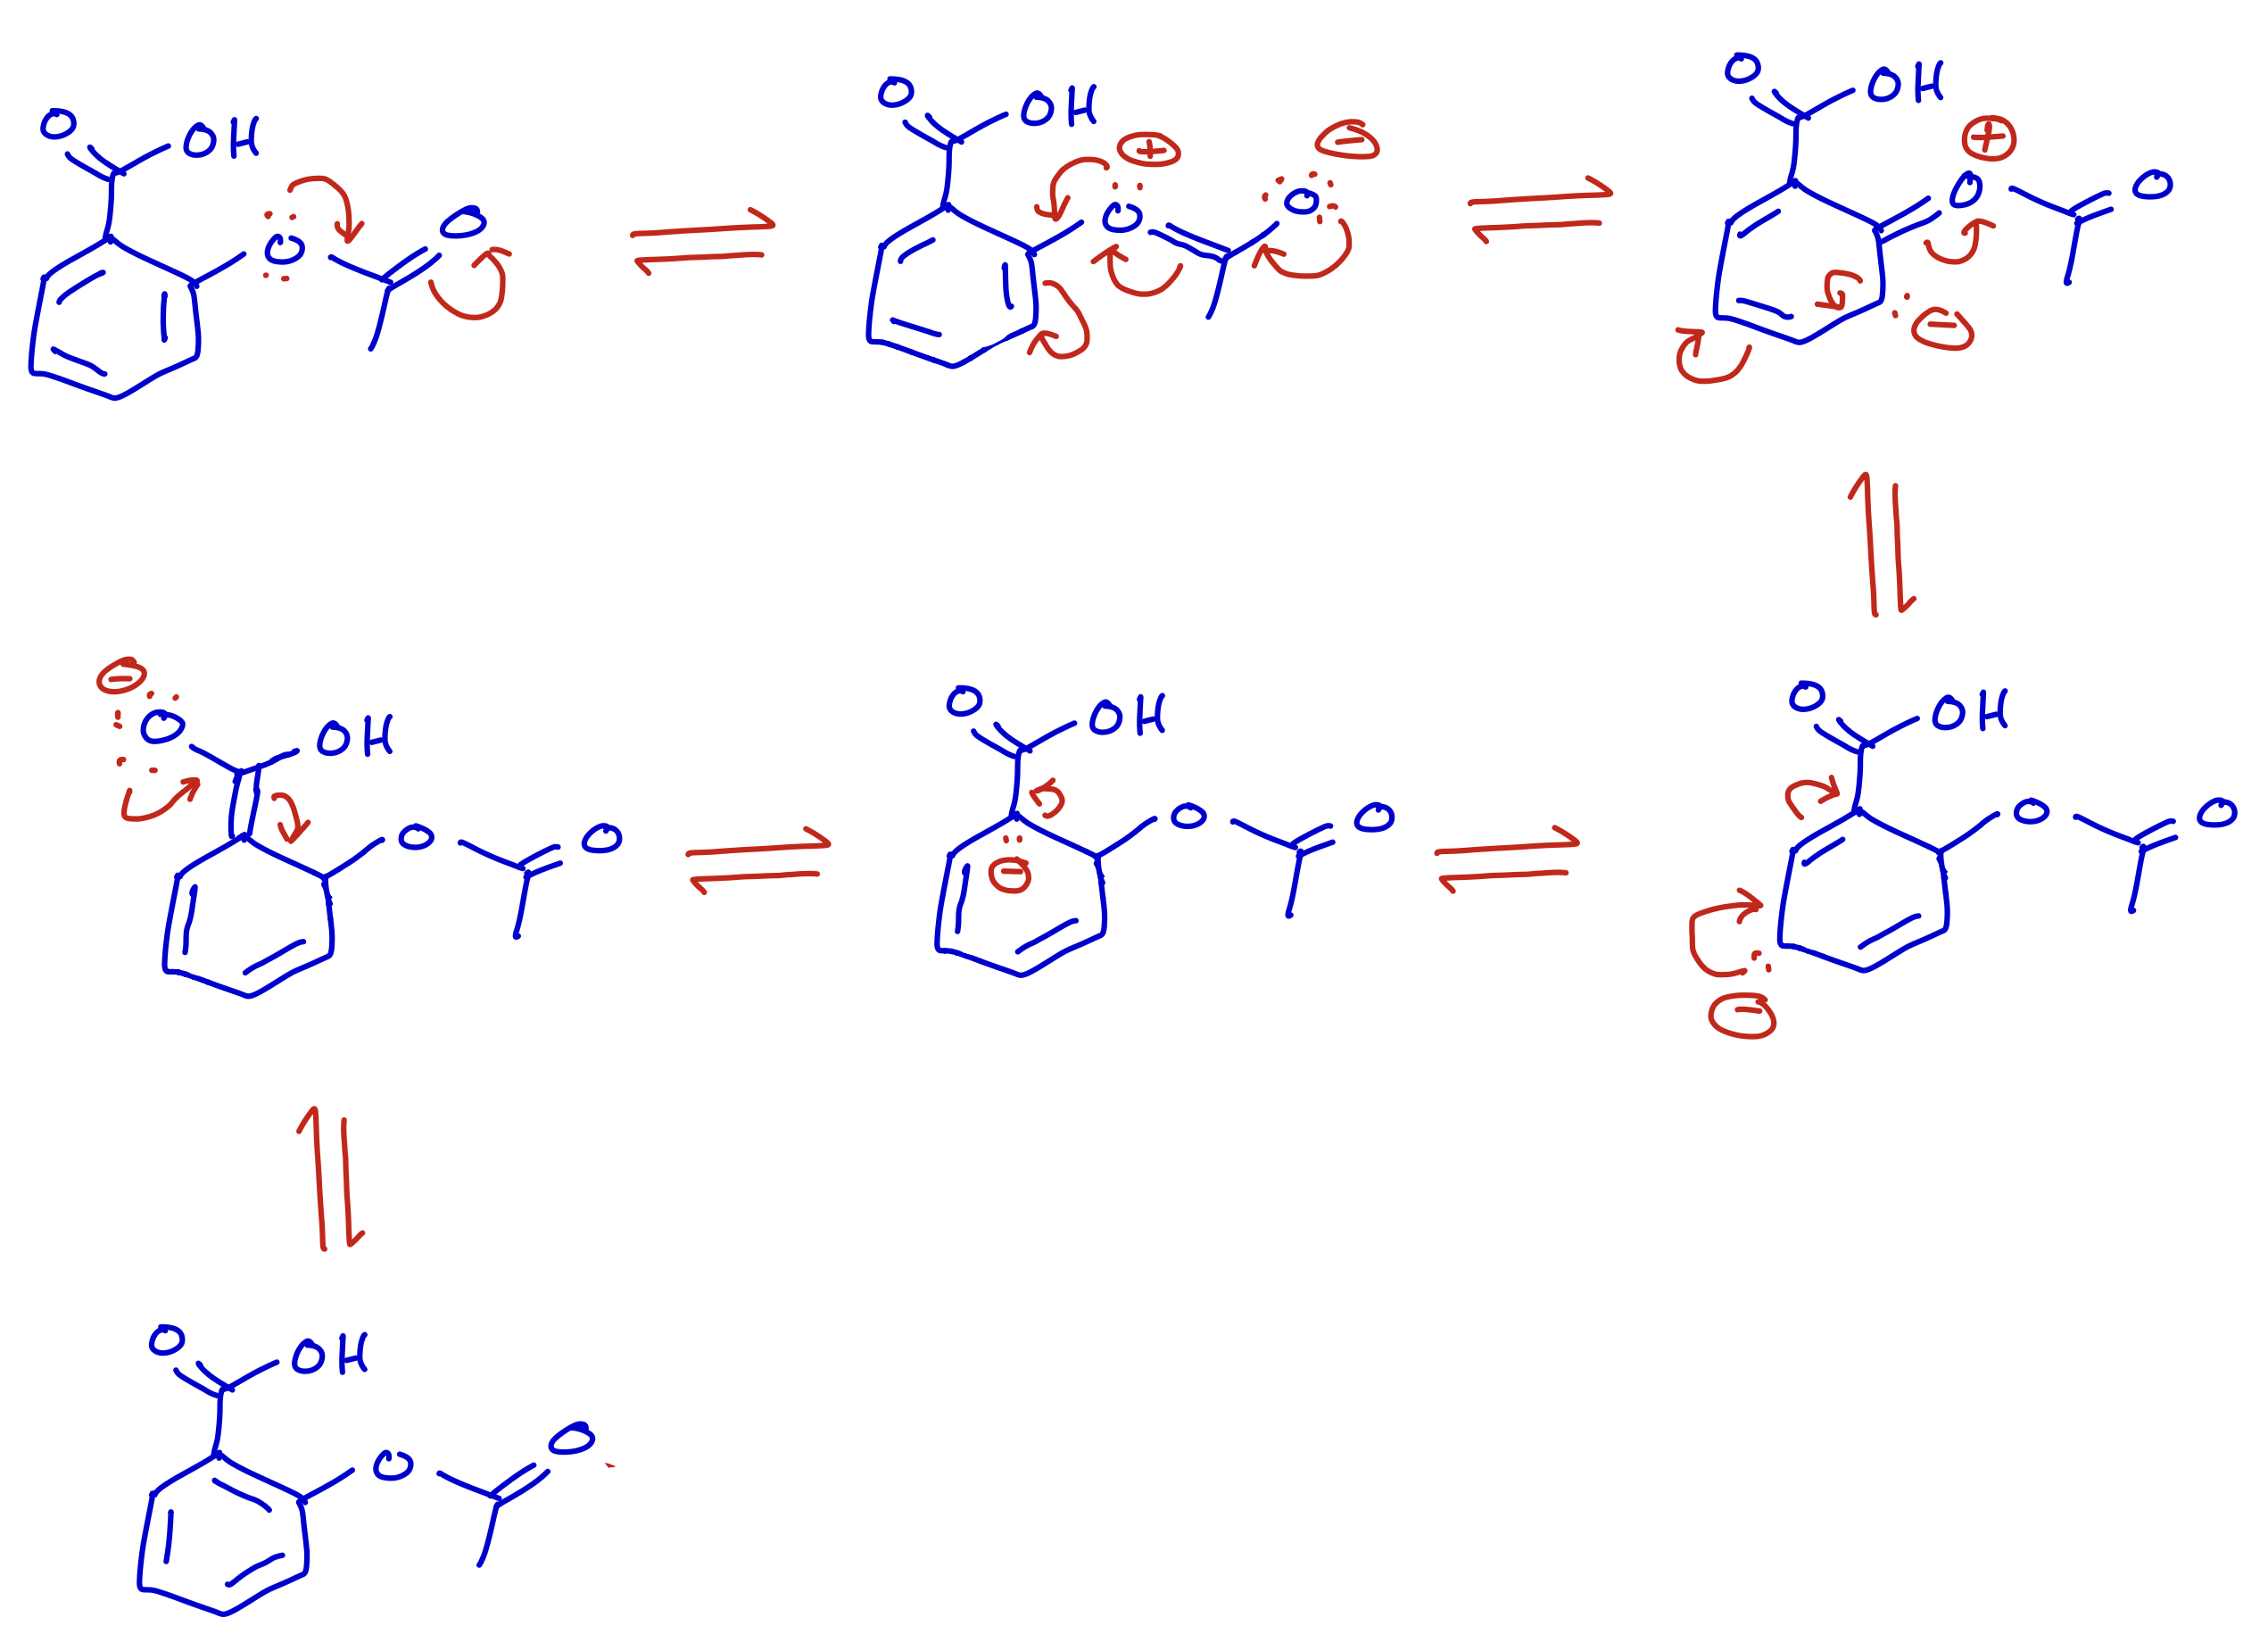
\includegraphics[width=0.56\linewidth]{img10.png}
\caption{CHEM~332\_Scheme~2. Resonance contributors of aspirin showing
acetoxy-oxygen lone-pair donation into the aromatic ring. The
$\pi$-donor character of the OAc group is what activates the C3 and C5
positions and makes it an o/p director in EAS, despite its
inductively electron-withdrawing $\sigma$ effect.}
\label{fig:resonance}
\end{figure}

\subsection*{Functional Groups}
Aspirin is a benzene ring bearing two ortho substituents: a
\textbf{carboxylic acid} (\(-\mathrm{COOH}\)) and an \textbf{aryl acetate}
ester (\(-\mathrm{OC(O)CH_3}\)). Counting the aromatic ring itself,
the molecule has three distinct functional groups, each of which
controls a different piece of its reactivity (Figure~\ref{fig:fg}).

\begin{figure}[H]
\centering
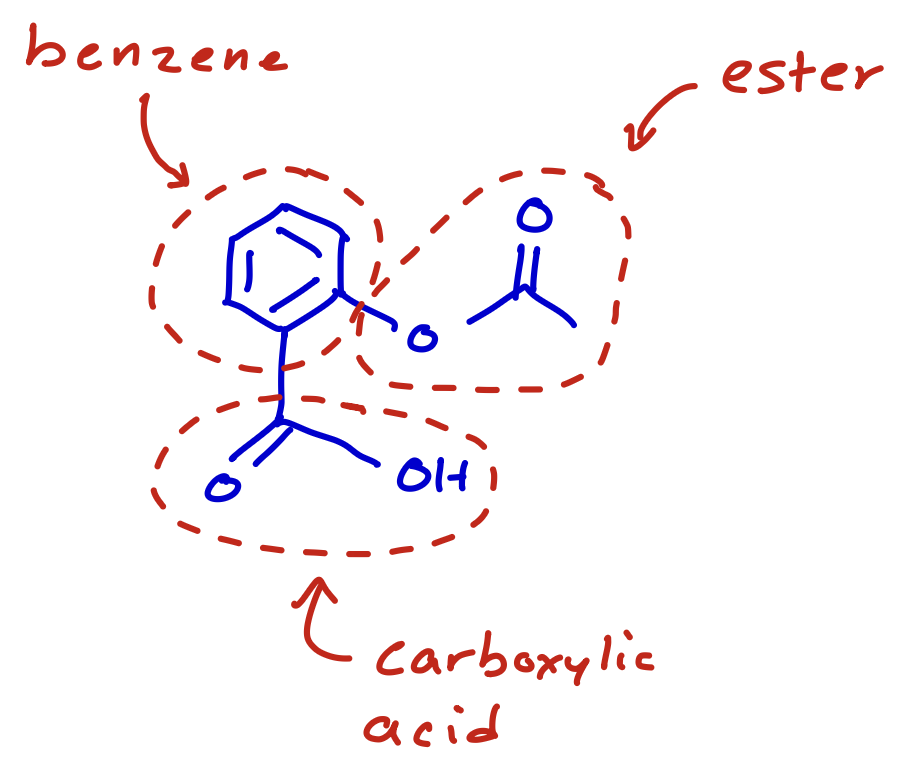
\includegraphics[width=0.32\linewidth]{img2.png}
\caption{CHEM~332\_Scheme~3. Functional groups in aspirin: the aromatic
ring (benzene), the aryl acetate ester at C2, and the carboxylic acid at C1.}
\label{fig:fg}
\end{figure}

\subsection*{Chiral Centers}
Aspirin has \textbf{no chiral centers}. No carbon in the molecule
carries four different substituents, so there are no stereocenters and
no $R/S$ configurations to assign; the molecule is achiral.

\section*{B. Synthesis Pathway}

The standard laboratory synthesis is the Fischer-type acylation of
salicylic acid with acetic anhydride under acid catalysis, with acetic
acid as the byproduct (Scheme~4). Conditions are typically
$50$--$60\,^\circ\mathrm{C}$ with a catalytic amount of concentrated
$\mathrm{H_2SO_4}$ (or $\mathrm{H_3PO_4}$ in the classroom version) and
a slight excess of acetic anhydride to push the equilibrium toward
product. After the reaction, the mixture is quenched with cold water,
which destroys the excess anhydride and precipitates the much
less-soluble aspirin for vacuum filtration and recrystallization from
ethanol/water.

\begin{figure}[H]
\centering
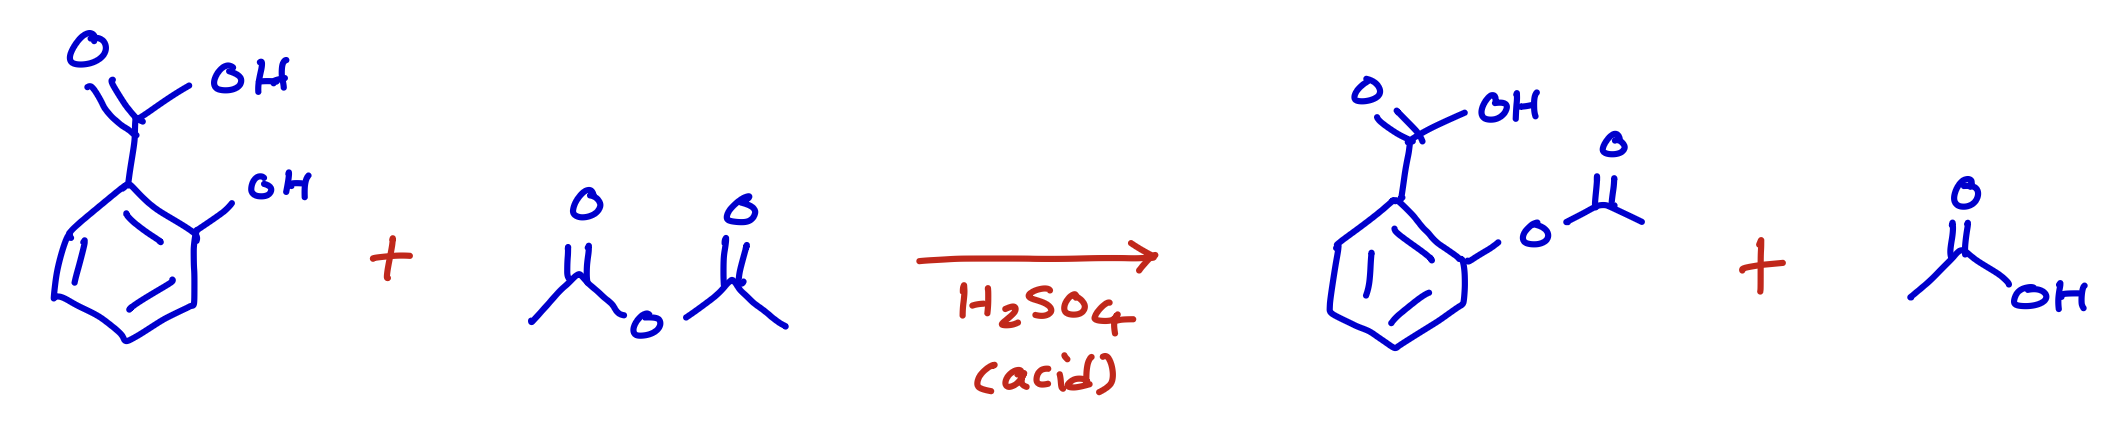
\includegraphics[width=0.6\linewidth]{img3.png}
\caption{CHEM~332\_Scheme~4. Overall reaction:
salicylic acid $+$ acetic anhydride $\xrightarrow{\;\mathrm{H_2SO_4}\;}$
aspirin $+$ acetic acid.}
\label{fig:synthesis}
\end{figure}

The reaction proceeds in three mechanistic stages. To save space the
acid catalyst is abbreviated $\mathrm{HA}$.

\subsection*{Activation of Acetic Anhydride}
The acid protonates one of the carbonyl oxygens of acetic anhydride.
This raises the LUMO of the carbonyl carbon and turns the anhydride
into a much better electrophile (Figure~\ref{fig:mech1}). Without this
activation the phenolic \(-\mathrm{OH}\) of salicylic acid is too weak
a nucleophile to react at a useful rate.

\begin{figure}[H]
\centering
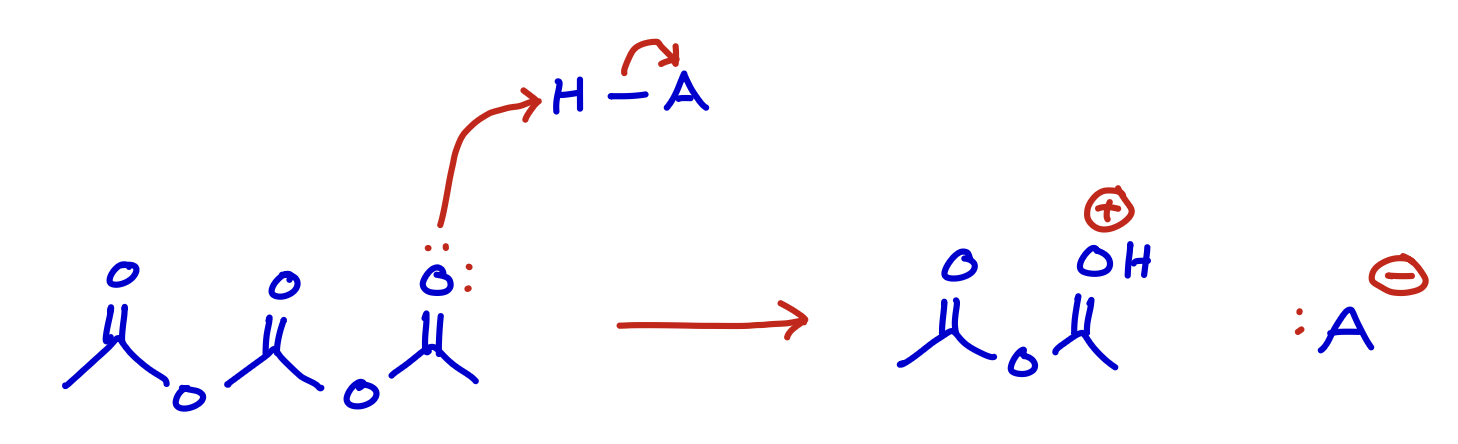
\includegraphics[width=0.5\linewidth]{img4.png}
\caption{CHEM~332\_Scheme~5a. Acid activation of acetic anhydride.}
\label{fig:mech1}
\end{figure}

\subsection*{Nucleophilic Attack by Salicylic Acid}
The phenolic oxygen of salicylic acid attacks the activated carbonyl
carbon, producing a tetrahedral intermediate. The conjugate base of the
catalyst removes the resulting oxocarbenium proton
(Figure~\ref{fig:mech2}). Note that the phenolic \(-\mathrm{OH}\) reacts
preferentially over the carboxylic \(-\mathrm{OH}\): the carboxylic
oxygen lone pairs are tied up in resonance with the adjacent
\(\mathrm{C{=}O}\) and so are less nucleophilic.

\begin{figure}[H]
\centering
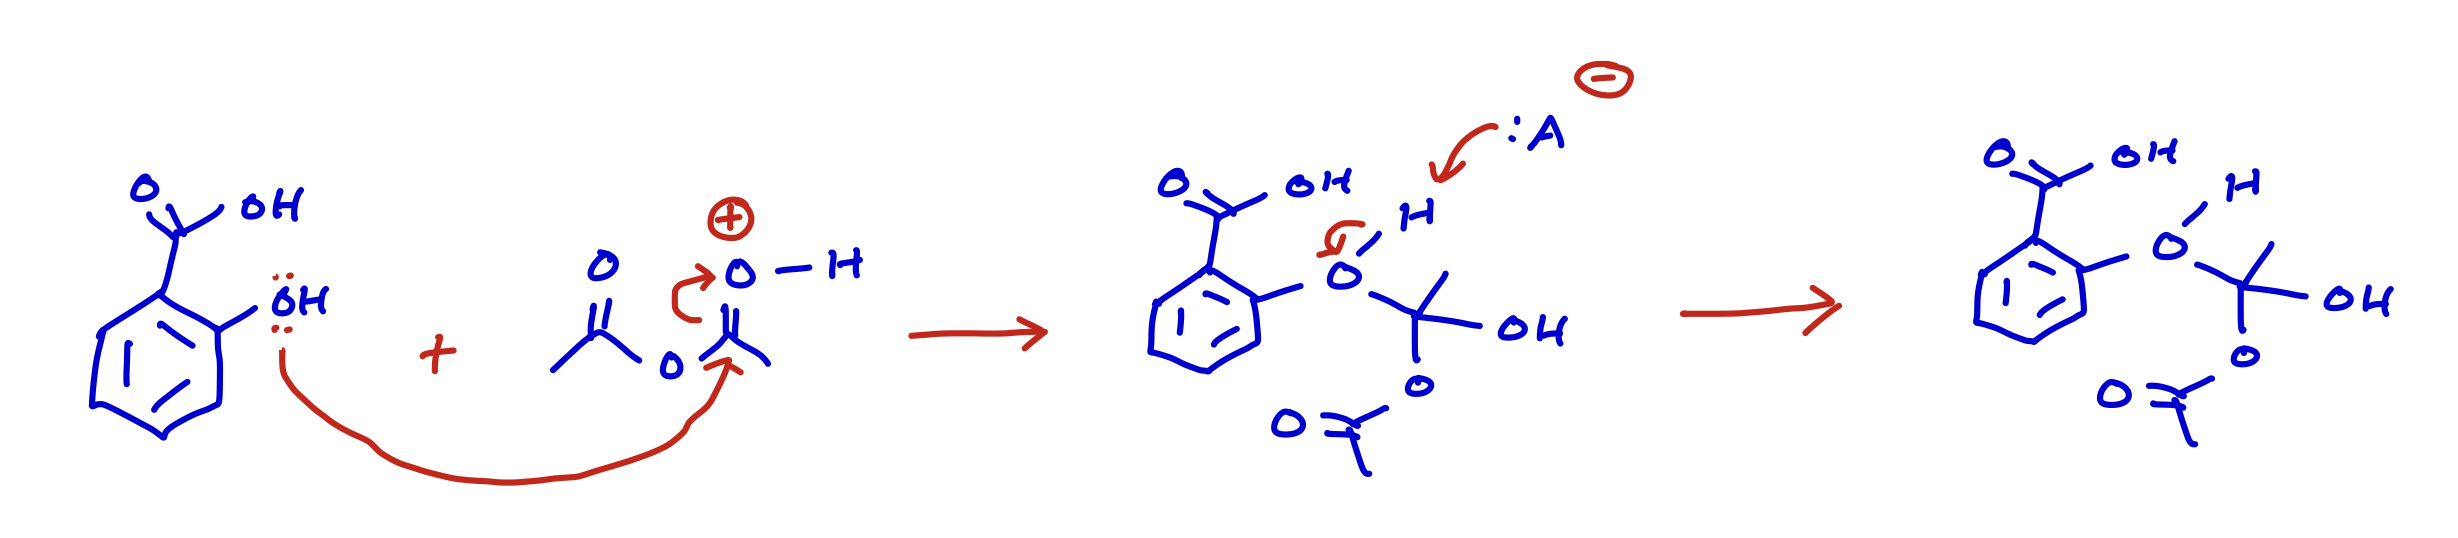
\includegraphics[width=0.6\linewidth]{img5.png}
\caption{CHEM~332\_Scheme~5b. Nucleophilic addition of salicylic acid
onto the activated anhydride to give the tetrahedral intermediate.}
\label{fig:mech2}
\end{figure}

\subsection*{Acetate as a Leaving Group and Deprotonation}
A proton transfer onto the acetate leaving group converts it into
neutral acetic acid; collapse of the tetrahedral intermediate then
expels acetic acid and regenerates the carbonyl. A final deprotonation
yields aspirin and returns the catalyst (Figure~\ref{fig:mech3}). The
acid is therefore strictly catalytic: it is consumed in step~1 and
regenerated by the end of step~3.

\begin{figure}[H]
\centering
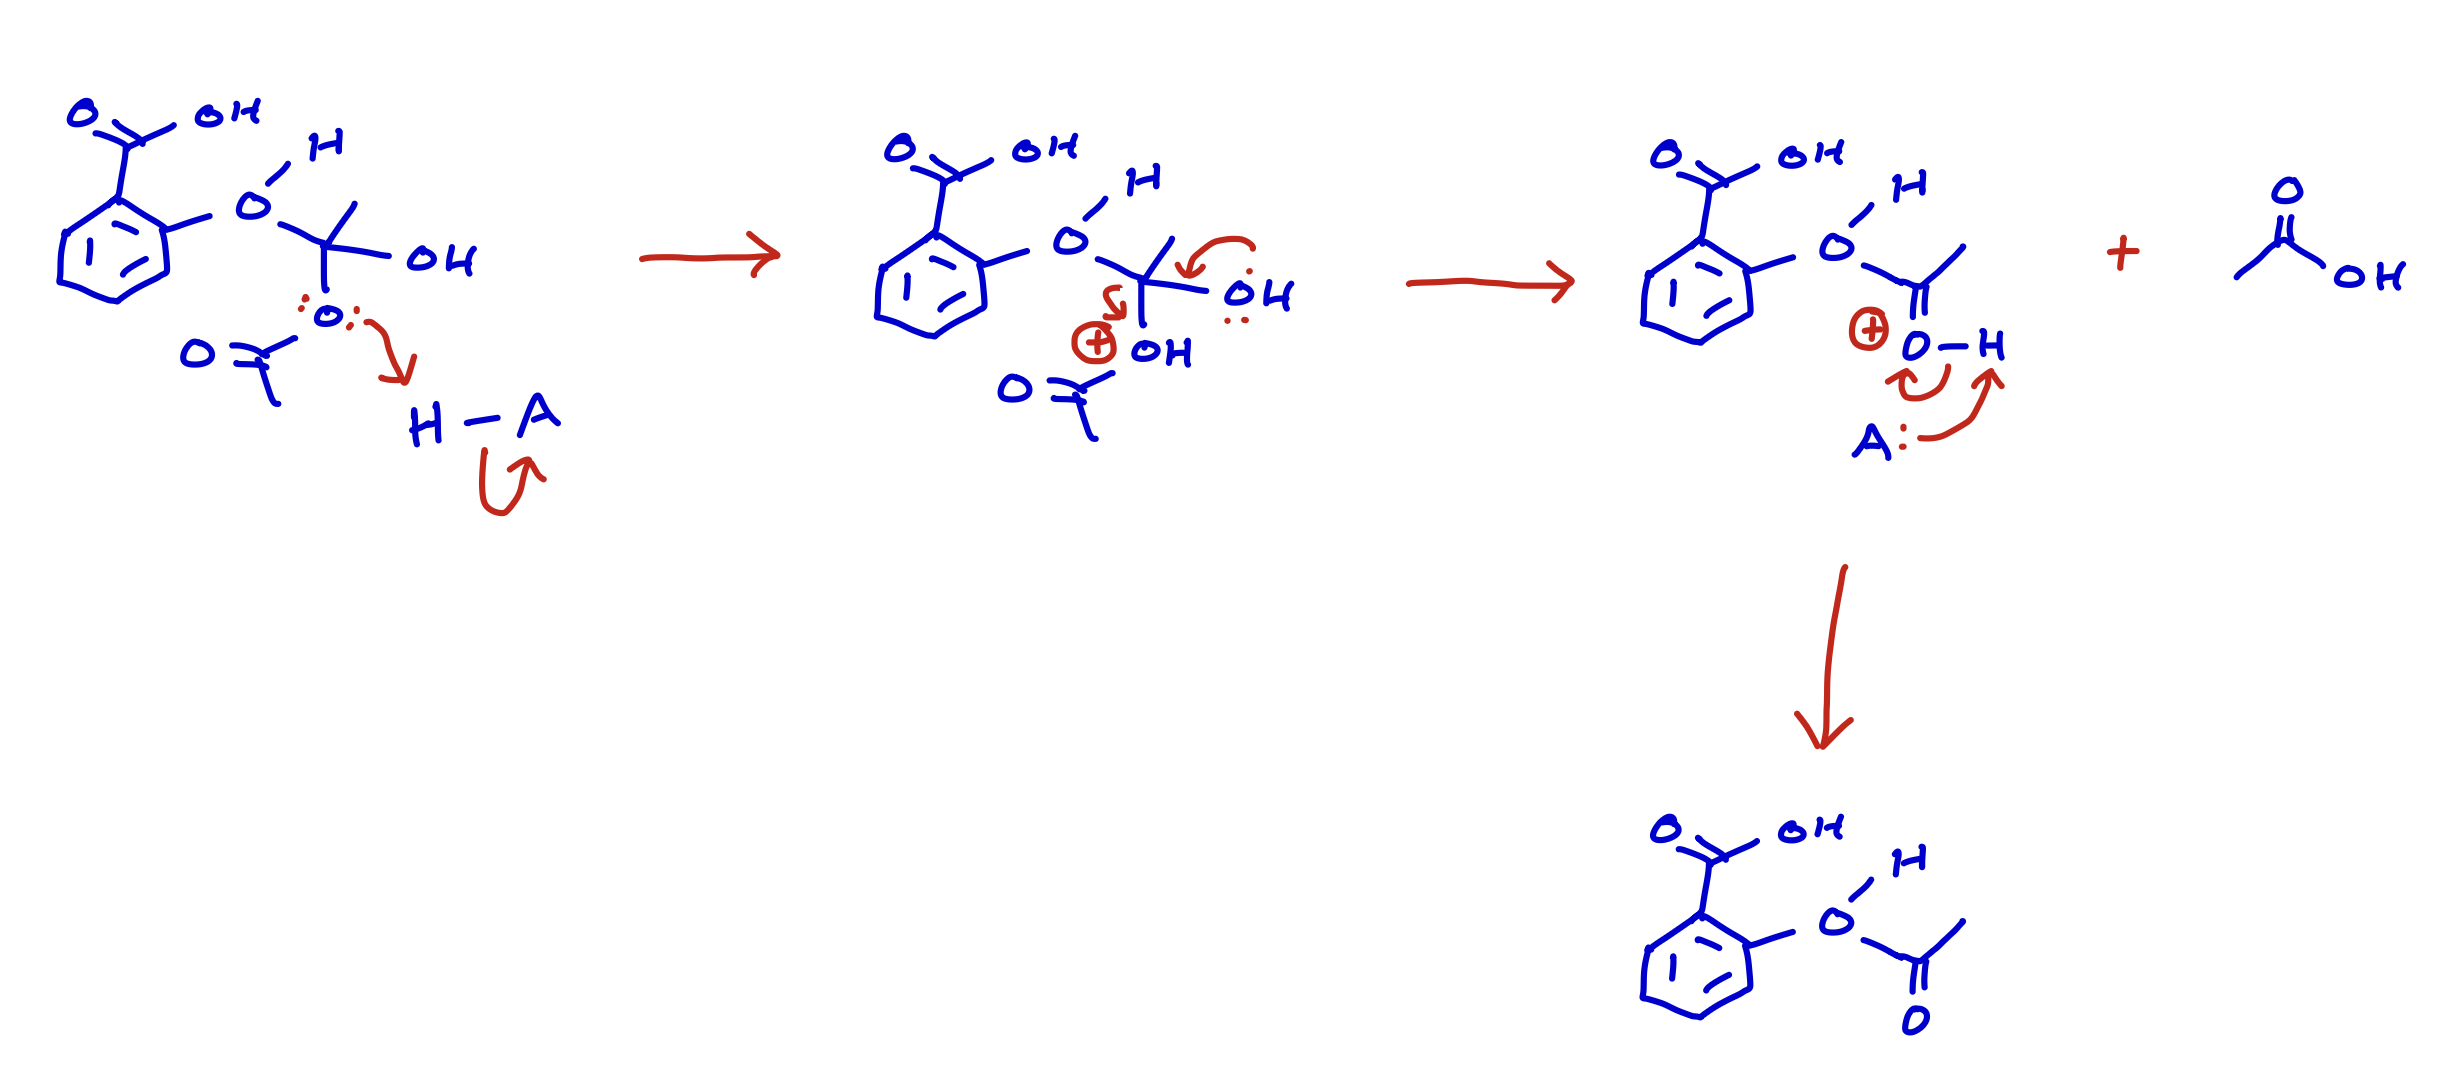
\includegraphics[width=0.66\linewidth]{img6.png}
\caption{CHEM~332\_Scheme~5c. Proton transfer, collapse of the
tetrahedral intermediate, and expulsion of acetic acid to deliver
aspirin.}
\label{fig:mech3}
\end{figure}

\section*{C. Functional Group Reactivity}

Each of aspirin's three functional groups has one characteristic
reaction from Organic I/II. The base-catalyzed hydrolysis of the ester
(below) is also the reaction I work through in detail with a full
mechanism, because it is mechanistically identical to the COX-1
acetylation step in Section~D.

\subsection*{Ester -- Hydrolysis}
The acetyl ester undergoes both acid- and base-catalyzed hydrolysis
back to salicylic acid and acetic acid; this is what limits aspirin's
shelf life in humid storage and in aqueous formulations.
Mechanistically (Figure~\ref{fig:hydrolysis}): (1)~$\mathrm{HO^-}$
attacks the electrophilic ester carbonyl, breaking the
\(\mathrm{C{=}O}\) $\pi$ bond and forming a tetrahedral alkoxide;
(2)~the alkoxide collapses, reforming the carbonyl and expelling
salicylate as the leaving group (a competent leaving group because the
resulting negative charge is stabilized both inductively by the
adjacent ring carboxyl and by delocalization into the ring); (3)~a
fast acid--base equilibration delivers neutral salicylic acid and
acetic acid. Under basic conditions the reaction is overall
irreversible because acetate is deprotonated to its conjugate base, so
acid-catalyzed re-esterification cannot restart the cycle.

\begin{figure}[H]
\centering
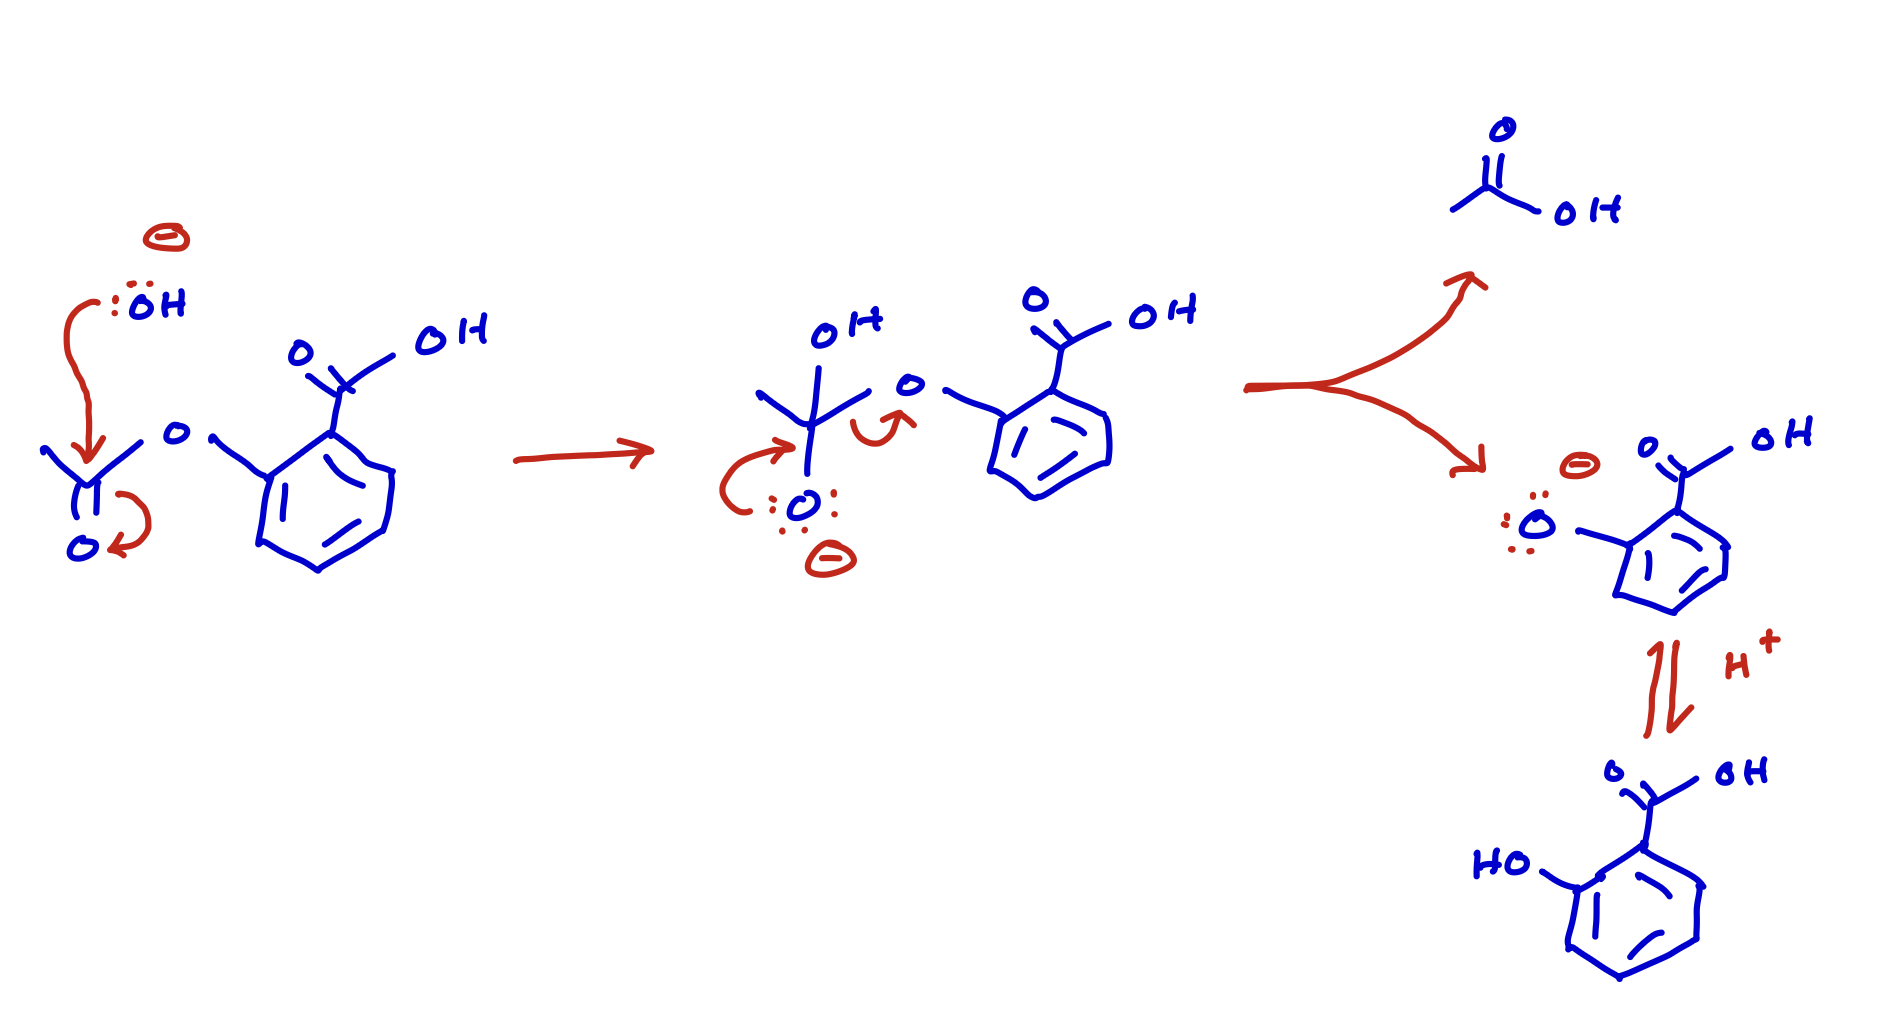
\includegraphics[width=0.62\linewidth]{img7.png}
\caption{CHEM~332\_Scheme~6. Base-catalyzed hydrolysis of aspirin's
acetyl ester: (1)~$\mathrm{HO^-}$ attacks the ester carbonyl, giving a
tetrahedral alkoxide; (2)~collapse expels salicylate and gives
acetate; (3)~proton transfer delivers neutral salicylic acid and
acetic acid.}
\label{fig:hydrolysis}
\end{figure}

\subsection*{Benzene -- Electrophilic Aromatic Substitution}
The aromatic ring is overall deactivated relative to benzene (both
substituents are net electron-withdrawing inductively) but is still
capable of EAS. The two substituents direct cooperatively
(Figure~\ref{fig:eas-direct}): the carboxylic acid is an EWG /
meta-director, and the acetoxy is a weak $\pi$-donor / o,p-director
through its oxygen lone pair (the resonance shown in
Figure~\ref{fig:resonance}). Both substituents therefore activate the
same set of positions, and the \textbf{C5 position} (para to
$-\mathrm{OAc}$, meta to $-\mathrm{COOH}$) is the kinetically preferred
site because it sits furthest from the steric bulk of the two ortho
substituents.

\begin{figure}[H]
\centering
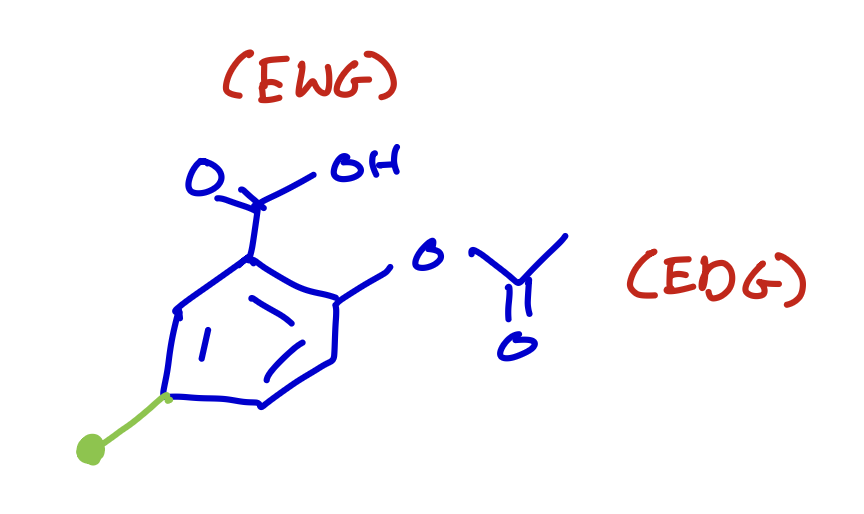
\includegraphics[width=0.32\linewidth]{img8.png}
\caption{CHEM~332\_Scheme~7. Directing analysis for EAS on aspirin.
$-\mathrm{COOH}$ (EWG, meta-director, top) and $-\mathrm{OAc}$ (weak
EDG, o/p-director, right) both activate the C3 and C5 positions; C5
(highlighted in green) is the kinetically preferred site.}
\label{fig:eas-direct}
\end{figure}

\subsection*{Carboxylic Acid -- Acid/Base Reactivity \& Deprotonation}
The $-\mathrm{COOH}$ group ($\mathrm{p}K_a \approx 3.5$) is
substantially deprotonated at physiological pH (7.4) to give the
carboxylate (Figure~\ref{fig:cooh}). The carboxylate is what dissolves
in plasma and what makes the electrostatic contact with Arg120 in the
COX active-site mouth (Section~D).

\begin{figure}[H]
\centering
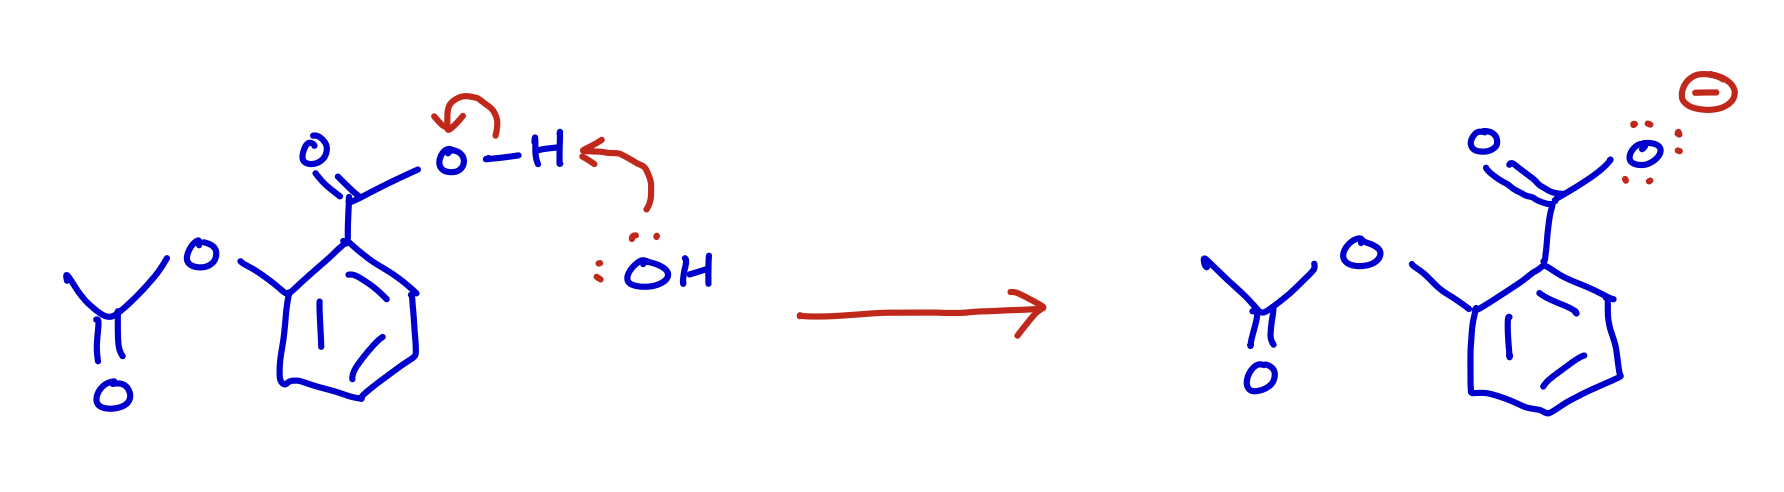
\includegraphics[width=0.42\linewidth]{img9.png}
\caption{CHEM~332\_Scheme~8. Acid--base reactivity of aspirin's
carboxylic acid: hydroxide deprotonates the $-\mathrm{COOH}$ to give
aspirin carboxylate (acetylsalicylate) and water.}
\label{fig:cooh}
\end{figure}

\section*{D. Biological / Pharmacological Role}

Aspirin's pharmacology is mechanistically tied to one specific reactive
feature of its structure: the \textbf{acetyl ester is a covalent
acetylating agent}. Aspirin diffuses into the active-site channel of
cyclooxygenase (COX-1 and COX-2), where Ser530 is positioned next to
the acetyl carbonyl. Ser530 nucleophilically attacks the carbonyl
carbon (essentially the same nucleophilic acyl substitution as the
hydrolysis step in Section~C), aspirin's acetyl group is transferred
onto the serine, and salicylate is released as the leaving group. The
serine is now permanently acetylated and cannot bind arachidonic acid,
so prostaglandin and thromboxane synthesis is blocked.

This explains aspirin's two clinical uses:
\begin{itemize}
  \item \textbf{Anti-inflammatory / antipyretic / analgesic.} Blocking
        prostaglandin H$_2$ synthesis lowers downstream PGE$_2$, which
        sensitizes peripheral nociceptors and drives the hypothalamic
        fever response. Less PGE$_2$ means less pain, less swelling,
        and a lower temperature set point.
  \item \textbf{Antiplatelet / cardioprotective.} Platelets cannot
        synthesize new protein, so once their COX-1 is acetylated they
        stay inhibited for their lifetime ($\sim$7--10 days). With
        thromboxane A$_2$ suppressed for that long, platelet
        aggregation is blunted -- the basis of the daily 81~mg ``baby
        aspirin'' regimen for secondary prevention of myocardial
        infarction and ischemic stroke.
\end{itemize}

The structural features driving this are exactly the ones identified
in Section~A: the ester provides the transferable acetyl group, the
carboxylate ($-\mathrm{COO^-}$ at physiological pH) anchors aspirin in
the polar mouth of the COX channel via Arg120, and the aromatic ring
orients the molecule so Ser530 sits in line with the acetyl carbonyl.

\section*{E. Safety and Environmental Impact}

\subsection*{Safety Concerns}
At therapeutic doses (325--650~mg for analgesia,
75--100~mg daily for cardioprotection) aspirin is well tolerated. The
most common adverse effect is gastrointestinal: by inhibiting COX-1 in
the stomach lining it reduces the protective prostaglandin layer and
raises the risk of gastric irritation, ulcers, and upper-GI bleeding
with chronic use. Salicylate overdose ($>$\,150~mg/kg) produces
tinnitus, mixed respiratory-alkalosis/metabolic-acidosis disturbance,
hyperthermia, and in severe cases coma; treatment is urinary
alkalinization with sodium bicarbonate and, if severe, hemodialysis.
Aspirin is also contraindicated in children with viral illness because
of the association with Reye's syndrome.

\subsection*{Environmental Impact}
Aspirin and its primary metabolite salicylic acid enter wastewater
through human excretion and improper
disposal. They are biodegradable and do not strongly bioaccumulate, but
chronic low-level exposure has been documented to cause oxidative
stress and histopathological changes in the livers of fish (e.g.\
\emph{Labeo rohita}) at environmentally relevant concentrations.
Aspirin is on the WHO Model List of Essential Medicines, and
manufacturing waste is regulated under standard pharmaceutical-effluent
rules.

\section*{F. Real-World Application}

In a February 2026 \emph{RSC Mechanochemistry} paper, Garumanna,
Thakuria, and Adassooriya prepared aspirin \textbf{nanocrystals}
($\sim$150~nm) by liquid-assisted ball-milling of bulk aspirin with
water at 30~Hz for 30~min, which is essentially a top-down,
solvent-minimal modification of the molecule's solid form rather than
its covalent structure. The nanocrystals released $\sim$90\,\% of the
drug within 6.5~min at simulated gastric pH ($\sim$1.2), versus
$\sim$50\,\% for bulk aspirin under the same conditions, and the
authors track a polymorph transition (Form~IV~$\rightarrow$ Form~I)
during milling. Practically, this matters because aspirin's oral
bioavailability is normally only $\sim$50\,\% on account of its poor
aqueous solubility -- a $\sim$3$\times$ acceleration of dissolution at
gastric pH is exactly the kind of formulation gain that translates into
faster onset of action without changing the chemistry of the molecule
itself.

\section*{References:}

\begin{enumerate}[label={[\arabic*]}]
\item Garumanna, G. D. S. K.; Thakuria, R.; Adassooriya, N. M.\
Mechanochemical synthesis of aspirin nanocrystals for pharmaceutical
applications. \emph{RSC Mechanochem.} \textbf{2026}, Advance Article.
\url{https://doi.org/10.1039/D5MR00118H}.

\item Vane, J. R.; Botting, R. M.\ The mechanism of action of aspirin.
\emph{Thrombosis Research} \textbf{2003}, \emph{110} (5--6),
255--258. \url{https://doi.org/10.1016/S0049-3848(03)00379-7}.

\item Awtry, E. H.; Loscalzo, J.\ Aspirin. \emph{Circulation}
\textbf{2000}, \emph{101} (10), 1206--1218.
\url{https://doi.org/10.1161/01.CIR.101.10.1206}.

\item Gayen, T.; Tripathi, A.; Kumari, U.; Mittal, S.; Mittal, A. K.\
Ecotoxicological impacts of environmentally relevant concentrations of
aspirin in the liver of \emph{Labeo rohita}: biochemical and
histopathological investigation. \emph{Chemosphere} \textbf{2023},
\emph{333}, 138921.
\url{https://doi.org/10.1016/j.chemosphere.2023.138921}.

\item Clayden, J.; Greeves, N.; Warren, S.\ \emph{Organic Chemistry},
2nd ed.; Oxford University Press: Oxford, 2012; Chapters 10
(carbonyl chemistry), 22 (electrophilic aromatic substitution).
\end{enumerate}

\section*{Reflections}

\textbf{1. Approach.}
I worked through the rubric in order so that each section could feed
into the next: structure first, then synthesis (to put the resonance
and functional-group analysis to use), then reactivity (which set up
Section~D's enzymology), and finally safety and recent literature.
Clayden, Greeves, and Warren was my main reference for the carbonyl
and EAS chapters, while Vane and Botting's COX-inhibition review
tied the pharmacology directly back to the acetylation chemistry I
had already drawn out. Drawing every figure in ChemDraw before
writing the prose forced me to commit to a mechanism early, which
made the prose much faster to write afterwards.

\textbf{2. Challenge.}
The hardest part was justifying the EAS regiochemistry, since
aspirin's two ring substituents are \emph{ortho} to each other and
push in different directions ($-\mathrm{COOH}$ is an EWG / meta
director while $-\mathrm{OAc}$ is a weak $\pi$-donor / o,p director).
I drew the $\sigma$-complex resonance forms for electrophile addition
at every ring position by hand and confirmed that only C3 and C5 keep
the positive charge off the carbon bearing $-\mathrm{COOH}$, with C5
ultimately favored on steric grounds. That exercise was the moment
EAS directing rules stopped being something I memorized and started
being something I could derive from the resonance picture.

\textbf{3. Key insights.}
The most useful realization was that the same nucleophilic acyl
substitution I drew for base-catalyzed ester hydrolysis (Section~C)
is exactly what COX-1 carries out on aspirin in vivo, with Ser530's
$-\mathrm{OH}$ playing the role of the nucleophile and salicylate
playing the role of the leaving group. Once that link clicked, the
pharmacology stopped being a separate list of clinical effects and
collapsed into one Organic~II mechanism applied to a much larger
molecule. The corollary was that ``drug design'' and ``reaction
mechanism'' are not separate disciplines for a molecule like aspirin
-- they are the same picture at different scales.

\textbf{4. Personal growth.}
This was the first time I had to make every chapter of Organic~I/II
agree on a single molecule simultaneously, which is a very different
exercise from solving a discrete homework problem. It pushed me to
treat reactivity as one continuous story driven by structure rather
than as independent textbook units, and to actually justify
conclusions (e.g.\ EAS regiochemistry, leaving-group ability) instead
of citing a rule of thumb. That habit of grounding every claim in a
mechanism is what I will carry into future chemistry and biochemistry
coursework.

\end{document}
